% Gemini theme
% See: https://rev.cs.uchicago.edu/k4rtik/gemini-uccs
% A fork of https://github.com/anishathalye/gemini

\documentclass[final]{beamer}

% ====================
% Packages
% ====================
\usepackage{amsfonts}
\usepackage[T1]{fontenc}
\usepackage{lmodern}
\usepackage[size=custom,width=30,height=48,scale=1.0]{beamerposter}
\geometry{paperwidth=30in,paperheight=48in}
\usetheme{gemini}
\usecolortheme{ucf}
\usepackage{graphicx}
\usepackage{booktabs}
\usepackage{tikz}
\usepackage{pgfplots}
\pgfplotsset{compat=1.17}

% ====================
% Lengths
% ====================

% If you have N columns, choose \sepwidth and \colwidth such that
% (N+1)*\sepwidth + N*\colwidth = \paperwidth
\newlength{\sepwidth}
\newlength{\colwidth}
\setlength{\sepwidth}{0.025\paperwidth}
\setlength{\colwidth}{0.3\paperwidth}

\newcommand{\separatorcolumn}{\begin{column}{\sepwidth}\end{column}}

% ====================
% Title
% ====================

\title{\textbf{$1^{st}$} Annual Research Symposium 2023 \\
``Rapid  and Accurate  INS Transfer Alignment \\ for Air  Launched Tactical Missile\\ Using  Kalman  Filter''}

\author{Sambhav  Kumar  Jain, Tapan  K.  Jain}

\institute[IIITN]{ \textit{Indian Institute of Information Technology, Nagpur} }

% ====================
% Footer (optional)
% ====================


\footercontent{
  \href{https://iiitn.ac.in}{https://iiitn.ac.in} \hfill
  PhD Cell, IIIT Nagpur, August 2023 \hfill
  \href{mailto:skjain.drdl@gov.in}{skjain.drdl@gov.in}}
\begin{document}
\addtobeamertemplate{headline}{}
{
    \begin{tikzpicture}[remember picture,overlay]
      \node [anchor=north west, inner sep=3cm] at ([xshift=0.0cm,yshift=3cm]current page.north west)
      {
\includegraphics[height=12cm]{logos/ucf_logo2.png}}; % also try shield-white.eps
      \node [anchor=north east, inner sep=3cm] at ([xshift=1.0cm,yshift=3cm]current page.north east)
 {
\includegraphics[height=12cm]{logos/DRDO1.jpeg}};
    \end{tikzpicture}
}

\begin{frame}[t]
\begin{columns}[t]
\separatorcolumn

\begin{column}{\colwidth}

  \begin{block}{Abstract}
  
 An Inertial Navigation System (INS) independently measures the Position, Velocity, and Attitude (PVA) of the vehicle to navigate it towards the target. Since INS is a dead-reckoning system, it requires accurate initialization to provide the navigation (PVA) solution. In the case of an air-launched tactical missile, the aircraft navigation system (Master  INS) information is used to initialize accurately the missile  INS  (Slave  INS). Rapid transfer alignment is needed in today’s combat operation to converge slave INS initialization in the shortest possible time using aircraft navigation information. The transfer alignment consists of first initializing the missile INS and establishing a navigation solution (PVA) using the missile IMU rates and accelerations, then a Kalman filter is used to, estimate the errors between the  Slave  INS  and  Master  INS.  The proposed method’s simulation results show that a  tactical missile INS can be aligned to an acceptable accuracy in a very short time based on the aircraft’s attitude information and with natural maneuvers experienced during aircraft take-off.
 \end{block}

  \begin{block}{Introduction}

Inertial Navigation System (INS) integrated into the air-launched  tactical  missile  is  normally  a  low-accuracy  strap-down  INS.  The  missile  INS  (Slave  INS)  can  be initialized \cite{reddy2013advanced} using the Position, Velocity, and Attitude (PVA) of the Master INS (Aircraft)as measurements for the estimation filter. After initialization, the slave INS uses measured rates and accelerations along three orthogonal axes to propagate the weapon’s Position, Velocity, and Attitude (PVA) independently.


\lipsum
\begin{figure}
    \centering
    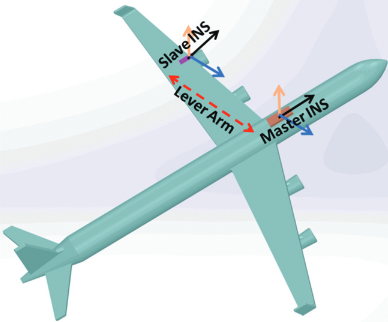
\includegraphics[width=1.0\textwidth]{logos/sambhav1.png}
    \caption{  Location of  Master  INS  and  Slave  INS  in a  typical aircraft-missile configuration (Lever arm).}
    \label{fig:img1}
\end{figure}
\lipsum

\par As shown in Figure 1, in a fighter aircraft Master INS is located at a location where the effect of the lever arm and vibration effect is minimum. Normally this location is along the aircraft axis.

\par Initializing the Slave INS, the Master INS information is communicated to the slave INS with ``nominal lever arm'' compensation as shown in Figure 2. The lever arm vector is the relative distance between the Master INS and the Slave INS. The lever arm compensation is necessary to account for the centripetal and vibration effects when aircraft performs a maneuver during alignment. This one-shot \cite{titterton2004strapdown} transfer of information is used to initialize the slave INS.

\lipsum
\begin{figure}
    \centering
    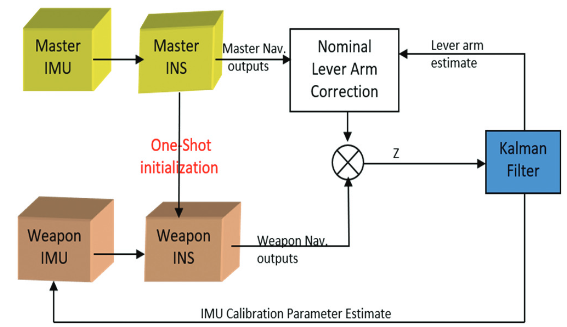
\includegraphics[width=1.0\textwidth]{logos/sambhav2.png}
    \caption{  Location of  Master  INS  and  Slave  INS  in a  typical aircraft-missile configuration (Lever arm).}
    \label{fig:img1}
\end{figure}
\lipsum

  \end{block}
  
  
  \begin{block}{About QIP Program}

The Government of India launched the 
 
\end{column}

\separatorcolumn

\begin{column}{\colwidth}

  \begin{block}{Course Objectives}
  
Machine learning algorithms are an integral part of almost all modern applications. To make the learning process faster and more accurate, a tool is needed which is flexible and powerful enough to help build machine learning algorithms quickly and easily. The workshop concentrates mainly on hands on exercises.
\\By the end of this workshop you'll not only have learned the difference between supervised and unsupervised models and their applications in the real world, but you'll also have developed the skills required to get started with programming your very own machine learning algorithms. 

  \end{block}

  \begin{block}{Topics to be Covered}
  
  Following topics to be covered:
  \begin{itemize}
  
 \item Introduction to AI/ML and ML algorithms
\item Decision trees and its practical applications

\item KNN, SVM, K means Clustering and its implementation
\item Neural Networks
\item CNN using Tensorflow and Keras
\item Moving Object Detection in a Video
\item Skin cancer detection using ML algorithms
\item Reinforcement Learning
\item Intrusion detection using ML algorithms
\item Diabetic retinopathy using Deep learning algorithms
\item IoT using ML
\item Introduction to NLP
\item Text classification using CNN
\item Predictive text analytics

\end{itemize}
  \end{block}
   \begin{alertblock}{Important Points}

    

    \begin{itemize}
      \item \textbf{Important Dates} Last date of online registration: March 04,2022.
      \item Intimation of participants: March 05,2022.

     
      \item No registration fee will be charged from the participants.
      \item Six days online mode Short term course
      \item Four sessions per day through Cisco Webex
      \item \textbf{Resource Person:}
Industry and academic experts from IITs, NITs and  IIIT will be the resource persons of the workshop. 
 \item \textbf{Registration:} Only online registration of participants to be done through a \underline{ \href{https://forms.gle/vudZyJhHLTd9Ufyt6}{google form}}\\
 
 \begin{figure}[h]
    \centering
    
\includegraphics[width = 0.3\textwidth]{logos/paperQR.png}
    \label{fig:my_zero}
\end{figure}
 
 \\ \newline



    \end{itemize}




  \end{alertblock}

\end{column}

\separatorcolumn

\begin{column}{\colwidth}
  \begin{block}{About the Course}
  

This workshop from leading researchers at different reputed Indian Universities introduces you to the exciting, high-demand field of Machine Learning. Through a series of practical case studies, you will gain applied experience in major areas of Machine Learning including Prediction, Classification, Clustering, and Information Retrieval. You will learn to analyze large and complex datasets, create systems that adapt and improve over time, and build intelligent applications that can make predictions from data.


  \end{block}

  \begin{block}{Eligibility}
  
 Applicants enrolled for M.Tech./Ph.D./PDF in a UGC recognized university/deemed university/AICTE approved colleges/institutes of national importance or Research Institutes only can apply for the workshop. The Specialisation of the applicant can be Engineering or interdisciplinary areas.

  \end{block}
  

\begin{block}{Conclusions}
\begin{itemize}
    \item The   main   objectives   of   the   proposed   scheme   are demonstrated  for  estimating  the  accurate  misalignment between Master and Slave INS and initializing the Slave INS with corrected Position, Velocity, and Attitude from Master INS.
    \item An  innovative provision without  the  need for  specific maneuver  and lever  arm  compensation,  the  accurate transfer  of  INS  information  demonstrated,  which  avoids the  need  for  extra  maneuver  on  combat  operation  by Aircraft pilot.
\end{itemize}

\end{block}
    \begin{block}{Acknowledgments}
The authors are extremely grateful to Dr. J Umakant, Mr. M. Kannan, Mr. R S Chandrasekhar and Mr. Sandeep Pal for sharing their knowledge, valuables ideas, and guidance which are immensely helpful in various stages of this work. The authors also like to express their deep sense of gratitude to Director DRDL, Director RCI, and Dean & Director IIIT Nagpur for giving motivation and opportunity to work on this problem.

\end{block}

\begin{block}{References}

\bibliographystyle{plain}
\bibliography{poster}

\end{block}
\end{column}

\separatorcolumn
\end{columns}
\end{frame}

\end{document}
